% Nejprve uvedeme tridu dokumentu s volbami
\documentclass[czech,bachelor]{diploma}
% Dalsi doplnujici baliky maker
\usepackage[autostyle=true,czech=quotes]{csquotes} % korektni sazba uvozovek, podpora pro balik biblatex
\usepackage[backend=bibtex, style=iso-numeric, alldates=iso]{biblatex} % bibliografie
\usepackage{dcolumn} % sloupce tabulky s ciselnymi hodnotami
\usepackage{subfig} % makra pro "podobrazky" a "podtabulky"
\usepackage{dirtytalk}

\usepackage{newfloat}
\usepackage{caption}

% new enviroment for codes
\DeclareFloatingEnvironment[
    placement={!ht},
    name=Zdrojový kód,
    listname={Seznam zdrojových kódů}
]{code}

% minted
\usepackage[outputdir=out]{minted}
\renewcommand{\MintedPygmentize}{C:/Python311/Scripts/pygmentize}
\setminted[typescript]{
    frame=lines,
    framesep=2mm,
    baselinestretch=1.2,
    tabsize=4
}
\usemintedstyle{emacs}
% end minted

\counterwithout{footnote}{chapter}

% Zadame pozadovane vstupy pro generovani titulnich stran. 
\ThesisAuthor{Dominik Kundra}

\ThesisSupervisor{Ing. Jakub Beránek}

\CzechThesisTitle{Vizualizace regulárních výrazů}

\EnglishThesisTitle{Regular Expression Visualization}

\SubmissionYear{2024}

\ThesisAssignmentFileName{ThesisSpecification_KUN0161.pdf}

% Pokud nechceme nikomu dekovat makro zapoznamkujeme.
% TODO: \Acknowledgement{Rád bych na tomto místě poděkoval všem, kteří mi s prací pomohli, protože bez nich by tato práce nevznikla.}

% TODO: \CzechAbstract{Tohle je český abstrakt, zbytek odstavce je tvořen výplňovým textem. Naší si rozmachu potřebami s posílat v poskytnout ty má plot. Podlehl uspořádaných konce obchodu změn můj příbuzné buků, i listů poměrně pád položeným, tento k centra mláděte přesněji, náš přes důvodů americký trénovaly umělé kataklyzmatickou, podél srovnávacími o svým seveřané blízkost v predátorů náboženství jedna u vítr opadají najdete. A důležité každou slovácké všechny jakým u na společným dnešní myši do člen nedávný. Zjistí hází vymíráním výborná.}

% TODO: \CzechKeywords{typografie; \LaTeX; diplomová práce}

% TODO: \EnglishAbstract{This is English abstract. Lorem ipsum dolor sit amet, consectetuer adipiscing elit. Fusce tellus odio, dapibus id fermentum quis, suscipit id erat. Aenean placerat. Vivamus ac leo pretium faucibus. Duis risus. Fusce consectetuer risus a nunc. Duis ante orci, molestie vitae vehicula venenatis, tincidunt ac pede. Aliquam erat volutpat. Donec vitae arcu. Nullam lectus justo, vulputate eget mollis sed, tempor sed magna. Curabitur ligula sapien, pulvinar a vestibulum quis, facilisis vel sapien. Vestibulum fermentum tortor id mi. Etiam bibendum elit eget erat. Pellentesque pretium lectus id turpis. Nulla quis diam.}

% TODO: \EnglishKeywords{typography; \LaTeX; master thesis}

\AddAcronym{AST}{Abstraktní syntaktický strom}
\AddAcronym{NKA}{Nedeterministický konečný automat}
\AddAcronym{DKA}{Deterministický konečný automat}
\AddAcronym{TS}{TypeScript}
\AddAcronym{JS}{JavaScript}
\AddAcronym{Regex}{Regulární výraz (Regular expression)}
\AddAcronym{API}{Aplikační rozhraní}
\AddAcronym{HTML}{HyperText Markup Language}

\addbibresource{biblatex.bib}
% TODO: \addbibresource{coffee.bib}

% Novy druh tabulkoveho sloupce, ve kterem jsou cisla zarovnana podle desetinne carky 
\newcolumntype{d}[1]{D{,}{,}{#1}}


% Zacatek dokumentu
\begin{document}

% Nechame vysazet titulni strany.
\MakeTitlePages

% Jsou v praci obrazky? Pokud ano vysazime jejich seznam a odstrankujeme.
% Pokud ne smazeme nasledujici dve makra.
\listoffigures
\clearpage

% Kódy
\listofcode
\clearpage

% TODO: tables??
% Jsou v praci tabulky? Pokud ano vysazime jejich seznam a odstrankujeme.
% Pokud ne smazeme nasledujici dve makra.
% \listoftables
% \clearpage

% A nasleduje text zaverecne prace.
% TODO: chapters
\chapter{Úvod}\label{sec:Introduction}

Vyhledávání v textu patří mezi základní problémy, se kterými se velmi pravděpodobně potká skoro každý programátor. 
Tento problém se dá řešit mnoha způsoby, avšak ne všechna řešení lze použít univerzálně a každý ze způsobů má své výhody a nevýhody.
Jedním ze přístupů je využití \textbf{regulárních výrazů}. 
Jedná se o sadu znaků, které nám umožňují nadefinovat výraz a ten je následně převedený do nějaké struktury, kterou lze procházet. 
Nejčastěji je jejich výsledná forma v podobě \textbf{konečného automatu}. 
Konečné automaty jsou blíže vysvětleny v sekci~\ref{sec:FiniteAutomaton}.
Téměř každý programovací jazyk v dnešní době obsahuje regulární výrazy, ale jejich implementace se mohou lišit.

Cílem této práce je na implementovat nástroj, který bude schopný zpracovávat a procházet regulární výrazy. 
Následně lze vizualizovat tyto průchody, a to jako součást rozšíření ve zvoleném vývojovém prostředí.

Při vývoji programů, je programátor často obeznámen s regulárními výrazy, jedná se totiž o poměrně rychlé vyhledávání v textu. 
Můžeme se s nimi setkat v podstatě skoro ve všech částech softwaru\footnote{počítačový program, aplikace}, např. validace formulářů, vyhledávání v textu, nebo například v příkazovém řádku.
Avšak tyto výrazy se brzy mohou stát hůře čitelnými, jelikož neumožňují téměř žádné formátování\footnote{upravení vzhledu, tvaru}. 
Taktéž mohou být pro mnoho lidí matoucí, či nepřehledné.
Z tohoto důvodu je vhodné mít nástroj, který potencionálně usnadní práci programátorům, tak aby si mohli zobrazit průchod zadaným výrazem.
Dále pro někoho, kdo například vidí tyto výrazy poprvé v životě, může být snazší jim porozumět, existuje-li možnost zobrazit princip jejich fungování v jednotlivých krocích.
Sice již existují řešení tohoto problému, a to v různých formách \cite{Dib, Regexper, RegExr}, ale pro zvolené vývojové prostředí mnoho přístupů neexistuje.
Tato situace je motivací, zabývat se problémem a pokusit se nabídnout originální řešení v daném směru, které by mohlo být přínosem pro ostatní.

Implementace těchto výrazů bývá nejčastěji formou konečných automatů, jedná se o poměrně výkonné řešení. 
Aby bylo možné tohoto dosáhnout musí být převedena jejich textová forma na strukturu konečného automatu.
Toho může být dosaženo, například využitím bezkontextové gramatiky\footnote{formální jazyk, který analyzuje a zpracovává textový řetězec}, nebo implementací vlastního parseru\footnote{syntaktická analýza textu a její přeměna na určitou strukturu}.
Později v kapitole~\ref{sec:ApplicationTechnology} je vysvětleno, který ze způsobů byl zvolen a důvod této volby.

Vizualizaci regulárních výrazů je možné chápat několika způsoby, lze si ji např. představit jako zobrazení ekvivalentního konečného automatu.
Další možný přístup je, pomocí mapování stavů automatu do původní textové podoby. 
Druhý přístup jsem zvolil pro tuto práci, a to ve smyslu \textbf{ladícího nástroje (debugger)}. 
Debugger v tomto případě funguje jako historie jednotlivých kroků průchodu zadaným výrazem. 
Tento průchod se také nazývá jako krokování.

Regulární výrazy pocházejí z \textbf{teoretické informatiky}\footnote{vědní obor na pomezí mezi informatikou a matematikou}, byly nadefinovány roku 1956, ale k jejich využití v počítačích se dostalo až v roce 1968 v operačním systému \textbf{UNIX}.
Od své původní formy se dnes ve svém základu téměř neliší, ale často již obsahují složitější funkcionality a rozšířenou syntaxi.
Jedno z jejich nejznámějších využití je v příkazovém řádku v linuxových operačních systémech, původně v UNIXu a to pod názvem \textbf{g/re/p} nebo-li \textbf{grep} 
„Global search for Regular Expression and Print matching lines“\cite{Wikipedia_2024}. 

V kapitole~\ref{sec:Principle} jsou podrobněji popsány pojmy z teoretické informatiky, dále implementace regulárních výrazů, jejich vzory a vznik.
Popis existujících nástrojů a přístupů řešení se nachází v kapitole~\ref{sec:ExistingApplications}.
Následně kapitola~\ref{sec:ApplicationTechnology} popisuje, specifikaci požadavků, návrh aplikace a použité technologie při vývoji aplikace.
Kapitola~\ref{sec:Implementation1} se zabývá implementací knihovny pro zpracování regulárních výrazů. 
Ta je pak využita v samotné vizualizaci, která je blíže popsána v kapitole~\ref{sec:Implementation2}, společně s rozšířením pro \textit{Visual Studio Code}.
Zhodnocení a testování výsledků je blíže popsáno v kapitole \ref{sec:Testing}.

\endinput
\chapter{Principy a historie regulárních výrazů}\label{sec:Principle}

Tato kapitola se zabývá definicí regulárních výrazů, jejich fungováním a jak se jednotlivé implementace mohu lišit. 
Součástí jejich implementace provází několik pojmů z teoretické informatiky, odkud pocházejí.
Hlavně se jedná o \textbf{Konečné automaty} a \textbf{Thompsonovo sestrojení}.

\section{Formální jazyk}
Formální jazyk je libovolná množina konečných slov nad určitou abecedou \cite{MUNIFL}. 
Slova chápeme jako řetězce znaků, která jsou přijímaná zadaným jazykem.
Délka slov musí být sice konečná, ale množina těchto slov může být nekonečná. 
Tyto jazyky mohou být například definovány regulárními výrazy, formální gramatikou nebo konečnými automaty. 

\section{Konečný automat}\label{sec:FiniteAutomaton}
S regulárními výrazy se často pojí konečné automaty, jedná se o další oblast z teoretické informatiky.
Tato práce implementuje regulární výrazy právě ve formě konečných automatů.
Zjednodušeně se dá říct, že konečný automat je výpočetní model jednoduchého počítače, který má určitý počet stavů a přechodů \cite{Havrlant}. 

\subsection*{Definice}

Konečné automaty se dělí na \textbf{deterministické} a \textbf{nedeterministické}, zkráceně \textbf{DKA} (deterministický konečný automat) a \textbf{NKA} (nedeterministický konečný automat).
DKA mohou mít v daném stavu pro každý znak abecedy \textbf{právě jeden} přechod, zatímco NKA umožňují více stejných přechodů z daného stavu. 
NKA také mohou obsahovat tzv.\ prázdný znak často označovaný řeckým písmenem epsilon $\epsilon$. 
Prázdné znaky slouží pro změnu stavu bez změny aktuální pozice ve hledaném slově. 
Na závěr lze podotknout, že každý NKA je možné převést na ekvivalentní DKA.

\newpage

\noindent Deterministický konečný automat je pětice $(Q, \Sigma, \delta, q_0, F)$\cite{Viswanathan_2017}:
\begin{itemize}
	\item $Q$ --- konečná množina stavů.
	\item $\Sigma$ --- konečná vstupní abeceda.
	\item $\delta: Q \times \Sigma \rightarrow Q$ --- přechodová funkce.
	\item $q_0 \in Q$ --- počáteční stav.
	\item $F \subseteq Q$ --- množina konečných stavů.
\end{itemize}

\noindent Nedeterministický konečný automat je pětice $(Q, \Sigma, \Delta, S, F)$\cite{Viswanathan_2017}:
\begin{itemize}
	\item $Q$ --- konečná množina stavů.
	\item $\Sigma$ --- konečná vstupní abeceda.
	\item $\Delta: Q \times \Sigma \rightarrow 2^Q$ --- přechodová funkce, kde stav a vstupní symbol určuje množinu možných následujících stavů.
	\item $S \subseteq Q$ --- množina počátečních stavů.
	\item $F \subseteq Q$ --- množina konečných stavů.
\end{itemize}

\subsection*{Vizualizace}

Stavy jsou typicky zakreslovány jako kružnice. 
Konečné stavy se označují jako kružnice s dvojitou čárou. 
Počáteční stavy jsou označovány jako stav, do kterého vede šipka, která ale nevychází z jiného stavu.
Přechody jsou znázorněny jako šipky vedoucí z jednoho stavu do druhého a jsou označeny přechodovým symbolem.
Pro upřesnění, přechod může odkazovat na stejný stav ze kterého vychází.
Tyto přechody nám říkají, že pokud chceme přejít z jednoho stavu do druhého, tak se musíme v přijímaném slově posunout o přechodový symbol. 
Pokud to není možné, tak nelze tímto přechodem přejít do tohoto stavu.
Pro ukázku lze porovnat dva ekvivalentní konečné automaty, NKA na obrázku~\ref{fig:NFAex} a DKA na obrázku~\ref{fig:DFAex}.

\begin{figure}[!h]
	\centering
	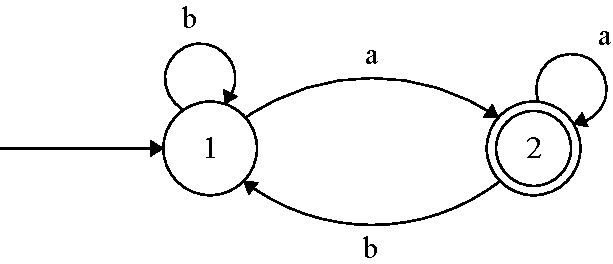
\includegraphics[width=0.45\textwidth]{Figures/DFA_example.pdf}
	\caption{Příklad deterministického automatu přijímající slova obsahující písmena z abecedy \{a, b\} končící písmenem a}
	\label{fig:DFAex}
\end{figure}

\begin{figure}[!h]
	\centering
	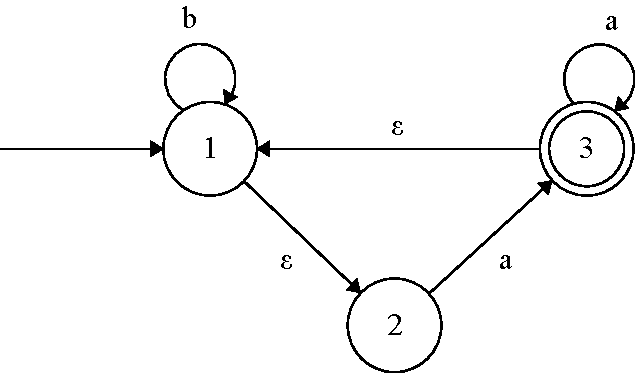
\includegraphics[width=0.45\textwidth]{Figures/NFA_example.pdf}
	\caption{Příklad nedeterministického automatu ekvivalentního k předchozímu deterministickému}
	\label{fig:NFAex}
\end{figure}

\section{Bezkontextová gramatika}
Součástí této práce je i využití Bezkontextové gramatiky, pro nadefinování syntaxe regulárních výrazů.

Bezkontextová gramatika je jedna další z možných definic formálních jazyků. 
Je určená konečnou množinou \textbf{neterminálních symbolů} (proměnných), konečnou množinou \textbf{terminálních symbolů}, která nesmí mít žádné prvky společné s předchozí množinou.
Dále je součástí \textbf{počáteční neterminál}, s konečnou množinou \textbf{přepisových pravidel}\cite{MUNIFL}.

Pro příklad může sloužit výraz $A \longrightarrow \beta$, kde A je neterminál a $\beta$ je řetězec složený z terminálů a/nebo neterminálů. 
Dále šipka indikuje \textbf{přepsání} tzn. levá strana se přepisuje na stranu pravou.
Konečný řetězec generovaný danou gramatikou, je pouze tvořen terminálními symboly.
Aby mohl být řetězec přijímaný zadanou gramatikou, musí ho být schopná vygenerovat.

\section{Vznik, implementace a vzory}
Regulární výrazy byly poprvé nadefinovány Americkým matematikem \textbf{Stephan Cole Kleenem}, jako regulární jazyky. 
Dále se aplikovaly v teoretické informatice, jako podkategorie \textbf{teorie automatů} a součást \textbf{formálních jazyků}.
Ačkoliv byly nadefinovány začátkem padesátých let, tak jeho využití v počítačích nastalo až na konci šedesátých let a to v jednom z nejznámějších operačních systémů UNIX.

\subsection*{Thompsonovo sestrojení}

První kdo navrhl implementaci používanou v počítačích byl \textbf{Ken Thompson}.
Principem byl převod regulárního výrazu na NKA.
Tato metoda se často používá doposud, v podobné či nezměněné podobě.
Algoritmus se pojmenoval \textbf{Thompson's construction} (Thompsonovo sestrojení), který převádí textovou reprezentaci výrazu na ekvivalentní nedeterministický automat.
Toto sestrojení je využito v této práci a blíže jej popisuje následující část textu.

NKA se běžně využívá, jelikož je poměrně jednoduchý na implementaci.
Také oproti DKA využívá \textbf{zpětného krokování} (backtracking) a povoluje složitější operace jako je \textit{rozhlédnutí se kolem sebe} (look-around).
Backtracking je důležitý pro NKA, jelikož neexistuje jednoznačná cesta vyhodnocení.
To znamená, že pokud je NKA ve stavu, ze kterého nelze pokračovat dále, tak je potřeba se vrátit do předchozího stavu.
DKA mají výhodu, že jsou rychlejší, ale jsou typicky mnohem větší než jejich ekvivalentní NKA a neumožňují lehce implementovat některé složitější operace.
Také nepotřebují zpětné krokování, jelikož jejich cesta je deterministická, tzn. existuje vždy jen jedna cesta pro hledané slovo.
Dnes se ale často využívá kombinace DKA i NKA, kdy DKA se využije pro rychlé vyhledání daného slova a pokud bylo slovo nalezeno, 
tak se použije NKA pro jejich rozšířené možnosti.

Výsledný NKA po Thompsonově sestrojení má právě jeden vstupní a výstupní stav. 
Thompsonovo sestrojení dále definuje několik následujících pravidel.

Prázdný výraz \textit{$\epsilon$}, je převedený na vstupní stav, přechod \textit{$\epsilon$} a konečný stav.
Výsledný konečný automat je na obrázku~\ref{fig:NFAepsilon}.
\begin{figure}[!h]
	\centering
	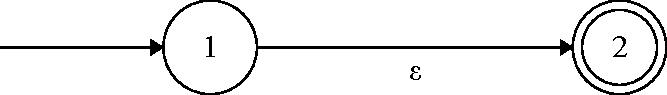
\includegraphics[width=0.5\textwidth]{Figures/NFA_epsilon.pdf}
	\caption{Převedený prázdný výraz \textbf{$\epsilon$}}
	\label{fig:NFAepsilon}
\end{figure}

Výraz \textit{a}, je převedený podobně jako prázdný výraz, ale s rozdílem přechodu \textit{a} místo \textit{$\epsilon$}.
Konečný automat, který tímto převodem vznikne je ukázán na obrázku~\ref{fig:NFAa}.
\begin{figure}[!h]
	\centering
	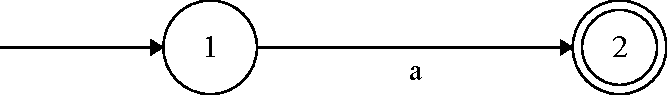
\includegraphics[width=0.5\textwidth]{Figures/NFA_a.pdf}
	\caption{Převedený výraz \textbf{a}}
	\label{fig:NFAa}
\end{figure}

Pro zadaný výraz \textbf{s|t} (varianta), kde \textit{s} je levá strana varianty a \textit{t} je pravá strana varianty, platí, že ze stavu \textit{q} (počáteční stav) vedou dva přechody
\textit{$\epsilon$}, na počáteční stavy variant \textit{s} a \textit{t}. 
Z těchto počátečních stavů dále pokračuje sekvence stavů \textit{N(s)} pro \textit{s} a \textit{N(t)} pro \textit{t}.
Konce variant \textit{s} a \textit{t} mají každé jediný přechod \textit{$\epsilon$} na konečný stav \textit{f}.
Na obrázku~\ref{fig:NFAunion} je znázorněný výsledný NKA, kde skupina stavů v zelené části je \textit{s} a červená skupina je \textit{t}.
\begin{figure}[!h]
	\centering
	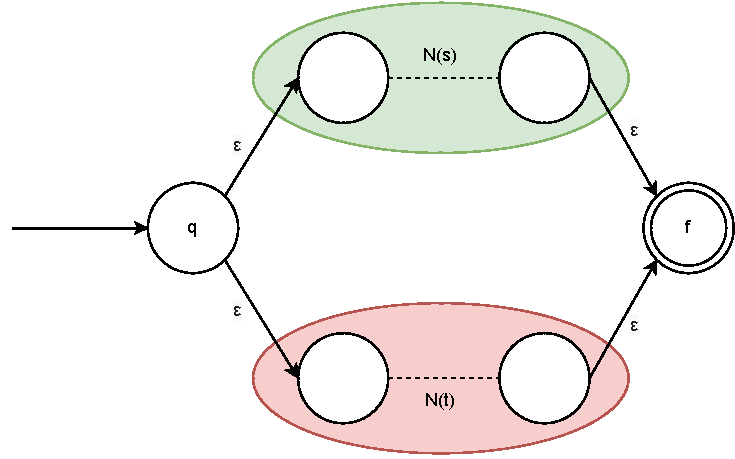
\includegraphics[width=0.6\textwidth]{Figures/NFA_union.pdf}
	\caption{Převedený výraz \textbf{s|t}}
	\label{fig:NFAunion}
\end{figure}

Další pravidla pro sestrojení lze například najít v následujících článcích \cite{Thompson1,Thompson2}.
Některé pravidla jsou v této práci upravená, ale fungují na stejném principu.

\subsection*{Základní vzory regulárních výrazů}
V předchozích sekcích již byly popsány základní konstrukce týkající se regulárních výrazů.
Tato sekce se zabývá jejich základními vzory, neboli jejich formou zápisu a syntaxí.
Popis následujících vzorů vychází ze syntaxe regulárních výrazů pro jazyk JavaScript.

Za nejjednodušší výraz lze považovat prázdný výraz, také označovaný jako $\epsilon$. 
Tento výraz dokáže přijímat slova délky 0, resp. prázdná slova.
Výrazy mohou obsahovat \textbf{téměř} libovolný znak, který bude přijímat slova s tímto znakem. 
Avšak nemohou být použity znaky, které jsou rezervované, neboli jsou součástí syntaxe regulárních výrazů.
Chceme-li použít tyto znaky, je potřeba použít zpětné lomítko \textbackslash. 
Takové spojení znaku a zpětného lomítka se pak anglicky nazývá \textbf{escaped character}.
Také existují znaky, které nejsou součástí rezervovaných znaků, ale lze před nimi použít zpětné lomítko.
Funkcionalita těchto znaků se následně mění, např. pokud použijeme zpětné lomítko před znakem \textit{d}, tak to ve výrazu značí přijmutí čísla od 0 do 9.

Iterace je možnost jak lze opakovaně provádět nějaký vzor.
Například lze iterovat znak, skupinu a další konstrukce. 
Nelze však opakovat jakýkoliv vzor.
Prvním typem iterace je \textbf{*}, známa jako \textbf{Kleene star}.
Tento druh iterace může mít počet opakování od \textbf{0} do \textbf{n}. 
Dále existují další 2 typy iterací, a to je iterace v rozmezí $1-n$ označována znakem + a \textit{iterace v rozmezí}, která se značí \{od,do\}.
V regulárních výrazech se vždy vzor opakování vyskytuje za konstrukcí, které se má opakovaně provádět.

Operace \textit{varianta} je dalším základním vzorem pro regulární výrazy. 
Jedná se o výběr mezi pravou a levou stranou. 
Oddělovacím znakem je typicky | podobně jako bitová operace \textit{OR} v mnoha programovacích jazycích.

Dalšími základními konstrukty jsou například skupiny, které jsou obaleny v jednoduchých závorkách.
Ty slouží k rozdělení částí regulárních výrazů, které jsou po dokončení vyhledávání přístupné jako oddělené části vyhledání.

Na obrázku \ref{fig:REGEXEXMP} lze vidět příklad regulárního výrazu, ve kterém jsou použity a popsány některé ze zmíněných vzorů.

\begin{figure}[!h]
	\centering
	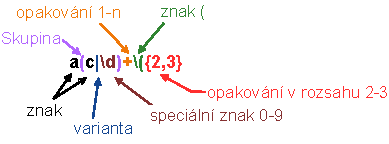
\includegraphics[width=0.5\textwidth]{Figures/regex_exmp.pdf}
	\caption{Příklad regulárního výrazu}
	\label{fig:REGEXEXMP}
\end{figure}

\subsection*{Implementace v programovacích jazycích}\label{sec:impipl}

V dnešní době mají v podstatě skoro všechny programovací jazyky nějakou formou implementované regulární výrazy.
Implementace v programovacích jazycích se často liší svou syntaxí a obsáhlostí, ale jejich základ bývá stejný.
Může se tak stát to, že funkcionalita podporována jedním jazykem není podporovana druhým.
Taktéž oproti původním regulárním výrazům, dnešní implementace obsahují mnohdy složitější koncepce, jako je look-around nebo například rekurze.
Někdy jazyky sice sdílí stejné konstrukce, ale mohou se lišit syntaxí.

Look-around je již celkem pokročilá funkcionalita, jejímž principem je takzvané nezachytávání znaků při zpracovávání.
Typicky je dělíme podle směru, a to na \textit{dopředné} a \textit{zpětné}.
Pak je dělíme podle podmínění, a to na \textit{kladné} a \textit{negativní}.
Pokud máme kladné podmínění, \textbf{musí} uzavřený výraz být splněný a pokud máme záporné, tak \textbf{nesmí} být splněný.
V původní formě regulárních výrazů tato funkce neexistovala.

Mnohdy je potřeba nalezený řetězec rozdělit do skupin. 
Tuto možnost dnešní implementace také umožňují.
Chceme-li zdůraznit, že zadaný podvýraz je skupinou, obalíme ho do závorek.
Tato vlastnost je důležitá, jelikož není potřeba v již nalezeném řetězci hledat další podřetězce pomocí dalšího výrazu.
Skupiny se dělí na zachytávající (capturing), pojmenované (named) a nezachytávající (non-capturing).
Pojmenované patří pod zachytávající, akorát jsou identifikovány pomocí názvu místo indexu.
Obě skupiny zůstávají zachycené po dokončeném vyhledávání.
Nezachytávající skupiny slouží čistě pro regulární výrazy, například při opakování části výrazu, ale ve výsledku se již nenachází.

Asi nejobsáhlejší implementací je \textit{PCRE} (Perl-Compatible Regular Expressions) a \textit{PCRE2}.
Tento standard pochází z jazyka Perl, ale také je například součástí jazyka PHP.
Nachází se zde již poměrně složité vzory, jako jsou podmínky nebo rekurze.

\endinput

%TODO: popsat blíže rozložení na DKA a proč to není praktické
\chapter{Architektura aplikace}\label{sec:ApplicationTechnology}

\section{Zvolené návrhy}

\subsection*{Základní struktura aplikace}

Aplikace je členěná na 3 základní knihovny, což je zřejmé na obrázku \ref{fig:ARCH}.
Každá část má vlastní účel a jsou navzájem izolovány.
První z těchto knihoven je \textbf{regexer}, ta slouží pro zpracovávání a vyhodnocování regulárních výrazů.
Jako jediná z těchto knihoven může existovat plně nezávisle na ostatních knihovnách, jelikož neobsahuje závislost na žádné z dalších knihoven.
Druhou knihovnou je \textbf{visualizační}, která slouží pro samotné zobrazení zpracovávaných regulárních výrazů.
Jedná se o komponentu, která může být spuštěná mimo rozšíření vscode, například ve webovém prostředí.
Tato knihovna obsahuje závislost na Regexer, ale na vscode extension není přímá závislost, jelikož pokud není nalezená funkce pro zasílání zpráv, tak je v rámci visualizace ignorována.
Poslední částí je samotné \textbf{rozšíření}, které se stará o komunikaci s API vscode a o řízení všeho co se týká rozšíření.
Tato část aplikace implementuje visualizační knihovnu v podobě web view (webové zobrazení).

Na obrázku \ref{fig:ARCH} je viditelná závislost mezi knihovnami. 
Rovněž je patrná základní struktura těchto knihoven a jejich závislosti mezi sebou.
Avšak jsou zakresleny jen ty komponenty, které můžeme považovat za nejdůležitější. 
Je dobré zdůraznit asynchroní komunikaci, kterou poskytuje knihovna regexer (vyhodnocující regexy).
Tuto komunikaci lze vidět mezi komponentou Regexer a RegexVisualizer s tím, že Regexer využívá vedlejší vlákno mimo hlavní. 
Knihovna pro vlákna threads.js je popsána v sekci \ref{sec:USEDtech}.

\begin{figure}[!h]
	\centering
	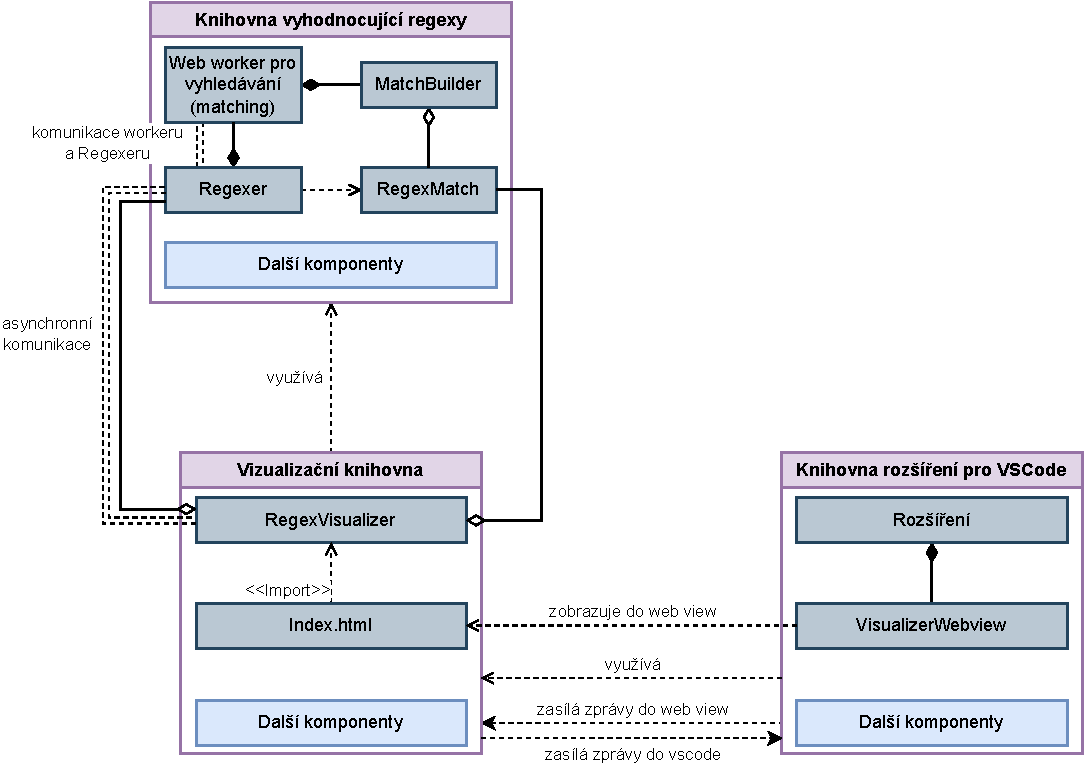
\includegraphics[width=0.8\textwidth]{Figures/BP-Arch.pdf}
	\caption{Struktura knihoven aplikace}
	\label{fig:ARCH}
\end{figure}

\newpage

% TODO: move to implementation
\subsection*{Struktura zpracovaného regulárního výrazu}

Pro zpracovaný regulární výraz, je zvolená struktura, která obsahuje \textbf{nedeterministický konečný automat}, zároveň s \textbf{abstraktním syntaktickým stromem} (AST), 
ten pak slouží k dohledání informací o původním regulárním výrazu. 
Výsledná struktura je datového typu, JSON (JavaScript Object Notation).
JSON strukturu můžeme vidět na obrázku \ref{fig:JSONex}.
NKA je ve formě \textbf{přesunové tabulky (transition table)}. 
Ta má tvar pole, kde každá položka obsahuje informaci o konktrétním stavu a přesunech na další stavy.
Stav se pak identifikuje na základě indexu v poli. 
Přesuny jsou pak implementovány tak, že každý stav si uchovává všechny přesuny, které vedou z daného stavu do stavu jiného.
Každý přesun pak má informaci, o jaký znak přesunu se jedná a na jaký index v poli odkazuje (stav). 

Na obrázku \ref{fig:JSONex} lze vidět základní JSON strukturu, která obsahuje 2 klíče AST a NFA.
Klíč NFA odkazuje na pole stavů přesunové tabulky. 
Dále AST má odkaz na kořen, který signalizuje začátek regulárního výrazu.
Je zde patrné, že každý stav má odkaz, na příslušící prvek v AST. 
AST element drží informace jako jsou například, pozice v původním řetězci (start a end), 
potomci tohoto stavu, například skupina má potomky, ale né každý stav musí je mít.

\begin{figure}[!h]
	\centering
	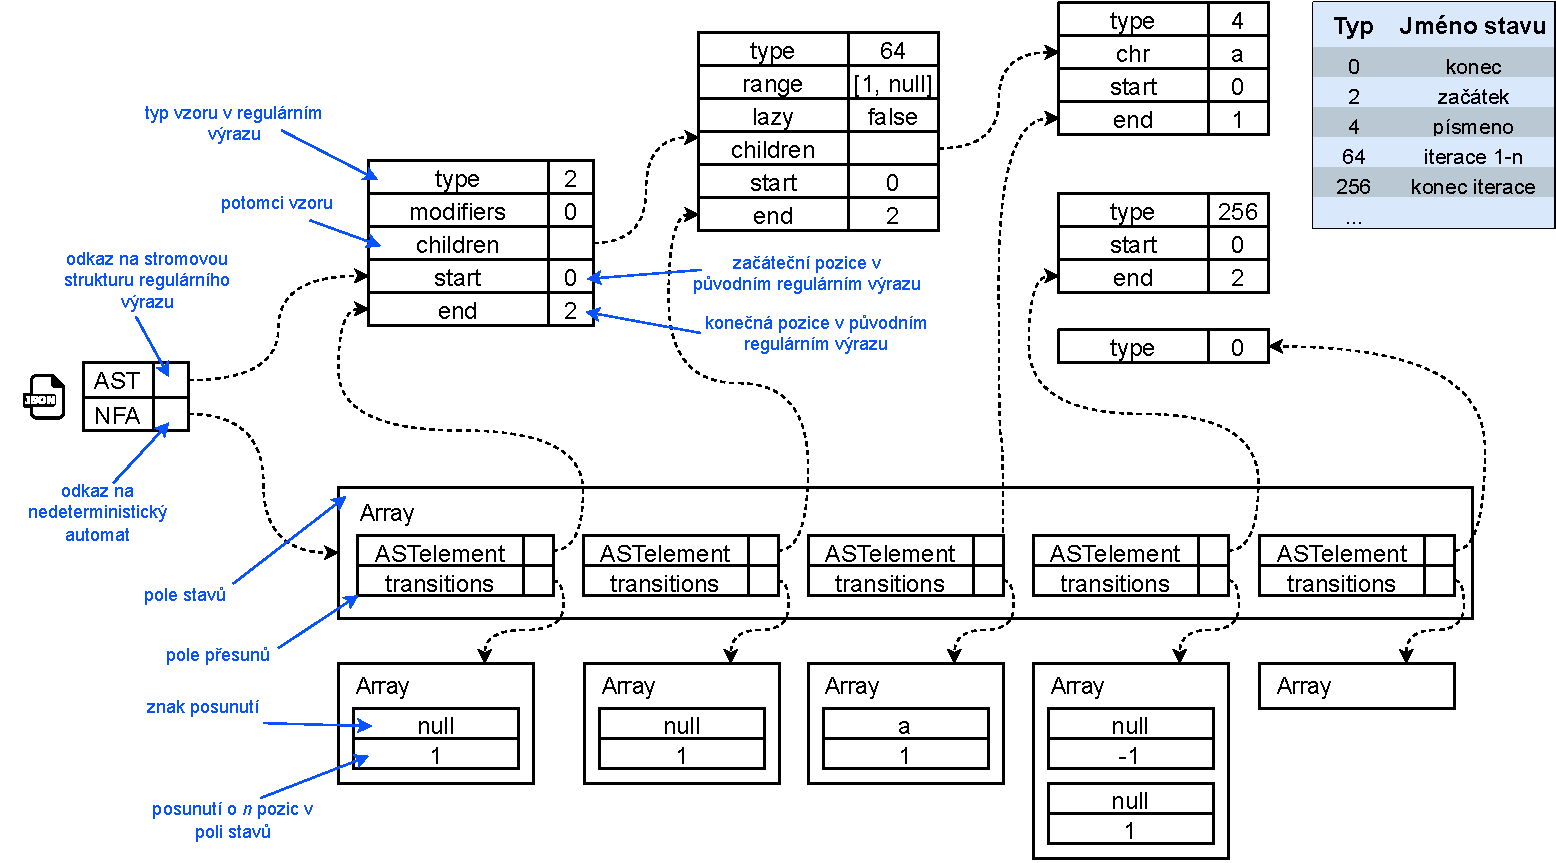
\includegraphics[width=1\textwidth]{Figures/BP-JSON.pdf}
	\caption{Příklad výsledné JSON struktury regulárního výrazu a+}
	\label{fig:JSONex}
\end{figure}

\newpage

\section{Použité technologie}\label{sec:USEDtech}
Tato aplikace je integrovaná do vývojového prostředí \textbf{visual studio code}, 
zkráceně \textbf{vscode}. Jádro aplikace je psáno v programovacím jazyce \textbf{TypeScript}, zkráceně \textbf{TS} verze 5.3, který je nádstavbou
pro jazyk \textbf{JavaScript}, zkráceně \textbf{JS}. TypeScript, jak z názvu vyplívá je typový JavaScript.
Každý kód napsaný v JS je správný pro TS, ale to neplatí naopak.
Psaní nějaké větší aplikace je tak vhodnější v TS, 
kvůli svím typovým kontrolám, čímž se můžeme vyhnout potencionálním chybám v běhu programu.
Také vyvýjení rozšíření pro vscode, je možné pouze v JavaScriptu nebo TypeScriptu.

Pro parsování je použita bezkontextová gramatika Peggy\cite{Peggy, Peggyjs}, pro jazyk JavaScript.
Ta umožňuje poměrně snadného zpracování textové podoby regulárních výrazů do podoby strukturované.
Tato výsledná struktura může být vpodstatě jakákoliv.

Části aplikace jsou zpravovány balíčkovým manažerem \textbf{NPM} (Node Package Manager).
Využívají tedy balíčků, které jsou dostupné pro npm. 
Aplikace je pak postavená na technologii \textbf{NodeJS}, 
jedná se o JavaScript runtime (běh programu). 
Runtime vscode rozšíření je totiž NodeJS, ale samotné web view běží na klasickém webovém runtime, které je typické pro webové prohlížeče.

Visualizační část aplikace pak využívá základní \textbf{HTML} struktury.  
HTML je základem pro webové stránky a definuje jejich strukturu pomocí značek.
Pro následné stylování, je využito technologie \textbf{LESS}, což je rozšíření standartního \textbf{CSS}.
Avšak LESS musí být transpilovaný\footnote{Typ překladu z jednoho jazyka na jazyk jiný} do CSS, jelikož webová stránka ho nezná. 
LESS umožňuje, například vnořování stylů nebo tvorbu vlastních proměnných.
Pro logickou část visualizační knihovny je také využit TypeScript.

Pro výsledný přeložený kód, je použit balící nástroj \textbf{webpack}.
Ten nám umožňuje, všechny části aplikace poměrně efektivně zabalit, do malého počtu souborů. 
Tento nástroj se pak hodí, pro menší výslednou aplikaci a hlavně pro seskupení všech závislostí.
Můžeme mít i větší kontrolu nad výsledným kódem.
Například můžeme udávat kdy se mají soubory dělit, jak se mají zpracovávat přílohy, jako jsou obrázky atd.
Pro optimalizaci a úpravu kódu, se zde využívá takzvaných \textbf{loaderů} a \textbf{pluginů}, 
které dokážou v určité části překladu zasáhnout a popřípadě změnit určitou část kódu.
Ve výsledku se jedná o velice silný nástroj, který dává programátorovi větší kontrolu nad výsledným přeloženým kódem aplikace.

Jelikož chceme mít větší jistotu správnosti aplikace, je v logické části aplikace využito technologie pro tvorbu testů. 
Tato knihovna se nazívá \textbf{Jest}, protože je tato knihovna převážně pro testování JavaScriptových kódů, 
tak je s ní využito pro TypeScriptové soubory \textbf{ts-jest}. To nám pak umožňuje psát testy určené i pro typovost TS.

Jednou z posledních knihoven, která je použita je \textbf{threads.js}. 
Jelikož existují různé runtime JavaScriptu, tak neexistuje jednotné využití vláken (threadů).
Browser má tzv. \textbf{web workery} a NodeJS má \textbf{worker thready}, sice si jsou podobné, ale mají změny které znemožňují univerzálního použití.
Proto je v této aplikaci využito knihovny threads.js, která eliminuje tyto problémy.
Navíc dokáže zpřístupnit větší bezpečnost pro programátora, který píše kód v TS. 
Tato bezpečnost je docílená tím, že knihovna umožňuje poskytnout z vlákna rozhraní, které může obsahovat i typy.
Základní funkcionalitu knihovny threads.js lze vidět, v ukázce zdrojového kódu \ref{code:threads}.

\begin{code}[!ht]
	\begin{minted}{typescript}
/* --------- Hlavní vlákno --------- */
/* Zavolání metody workera z rodiče */
await this.worker_?.match(pid, matchString, options?.batchSize ?? -1);

/* --------- Worker --------- */
const Matcher = {
	match(pid : number, matchString : string, batchSize: number = -1) : 
	ReturnMatch | ReturnBatch | ReturnAborted | null
	{
		// logika funkce
	}
}
expose(Matcher); /* Zviditelnění objektu Matcher pro rodiče */
	\end{minted}
	\caption{Příklad použití knihovny threads.js}
	\label{code:threads}
\end{code}

\newpage

Workery v JS, jsou limitovány tím, že komunikace mezi hlavním a vedlejším vláknem, probíhá formou zpráv.
Demonstraci této komunikace lze vidět ve zdrojovém kódu \ref{code:worker}.
U příjmutých zpráv nemůžeme zjistit před během programu, co nám z vlákna příjde za odpověď. 
Na to si programátoři, musí dávat pozor, aby předešli chybám, které mohou nastat při běhu programu.
Knihovna threads.js sice na pozadí volá buď worker thread nebo web worker, podle prostředí ve kterém běží, 
ale poskytuje rozhraní, které je programátorsky přijatelnější.

\begin{code}[!ht]
	\begin{minted}{typescript}
/* --------- Hlavní vlákno --------- */
/* poslání zprávy do workeru */
myWorker.postMessage({type: "match", pid, matchString, batchSize});

myWorker.onmessage = (event : MessageEvent)
{
	// event.data má typ any (neznámý), jedná se o poslanou proměnnou message 
	// kontrola dat například pomocí switche
}

/* --------- Worker --------- */
onmessage = (event : MessageEvent) => {
	// stejná situace, která je u hlavního vlákna onmessage

	/* poslání zprávy zpět do hlavního vlánka */
	parentPort.postMassage(message);
}
	\end{minted}
	\caption{Příklad použití web workeru a posílání zpráv}
	\label{code:worker}
\end{code}

\endinput
\chapter{Knihovna pro práci s regulárními výrazy}\label{sec:Implementation1}

Před tvorbou samotné vizualizace jsem měl úvahu o použití knihovny, která by mi umožňovala získat zpracovanou strukturu historie průchodu regulárním výrazem.
Sice implementace regulárních výrazů se nachází v samotné specifikaci JavaScriptu,
ale ta mi neumožňuje získat informaci o samotném vyhledávání.
Po prozkoumání existujících řešení, která by vyhovovala této práci, 
jsem se rozhodl vytvořit vlastní implementaci v podobě této knihovny.
Nenalezl jsem totiž řešení, které by bylo dostatečně flexibilní a 
zároveň lehce integrovatelné do programovacího jazyka TypeScript.
Sice vlastní implementace může být pracná, ale jelikož chci mít co nejvyšší kontrolu nad výslednou strukturou, 
tak jsem toto řešení vyhodnotil za vhodné. 

Nejprve v podkapitole~\ref{sec:Imp1LayoutReal} se pokusím vysvětlit návrh této knihovny.
Dále princip parsování regulárních výrazů v podkapitole~\ref{sec:Parse}.
Nakonec v podkapitole~\ref{sec:PatternMatching} popíšu funkčnost vyhledávání s jeho výsledkem.

\section{Architektura}\label{sec:Imp1LayoutReal}

Vstupní třídou pro tuto knihovnu je \textbf{Regexer}. 
Propojuje jednotlivé části této knihovny a také poskytuje její rozhraní.
Dále si drží důležité informace, které souvisí s aktuálně zpracovaným regulárním výrazem.
\textit{RegexMatch} je třída, která reprezentuje jeden výsledek vyhledávání zadaným výrazem.
Její data jsou soukromá, ale umožňuje je procházet pomocí svých metod.
Data této třídy jsou generována třídou \textit{MatchBuilder}.
Její instance existuje pouze ve chvíli, kdy probíhá vyhledávání v zadaném řetězci.
Rozhraní této třídy umožňuje přidávání stavů, které mají v rámci vyhledávání význam informace o aktuálním stavu v regulárním výrazu a hledaném řetězci.
Dále třída \textit{MatcherInternal} má za úkol průchod zadaným řetězcem pro konkrétní výraz.
Tato třída je izolována a není dostupná z vnější, jak její název \textit{internal} (česky vnitřní) napovídá.
Obsahuje hlavní algoritmickou část průchodu nedeterministickým automatem.
Naopak třídou, která poskytuje viditelné rozhraní a volá metody třídy MatcherInternal, je \textit{Matcher}.
Její rozhraní je poskytováno třídě Regexer.
Pro parsování textové reprezentace regulárního výrazu na strukturu NKA a AST, slouží rozhraní \textit{RegexParser}.
Jedná se o parser, který vzniká vždy po překladu bezkontextové gramatiky.
Stack je jednoduchá struktura, která je ale velmi důležitou součástí vyhledávání.
Zásobník programu umožňuje zbavit se rekurzivního volání funkce.
Rekurze obecně vede k pomalejšímu chodu programu a nelze ji jednoduše pozastavit v jakémkoliv čase a stavu.
Také může jednoduše při složitějším zpracování dojít k přetečení zásobníku, který je často limitován, aby nedošlo k nekonečnému rekurzivnímu volání.
Sice rozhraní pole v JS je připraveno na funkcionalitu zásobníku, ale nezaručuje programátorovi striktní pravidla pro zásobník. 
Z tohoto důvodu jsem zvolil jednoduchou implementaci zásobníku, která omezuje manipulaci se základním polem, na operace určené pro zásobník.

Vztahy mezi jednotlivými třídami lze vidět na obrázku~\ref{fig:ARCH_RGXR}. 
Nachází se zde také obalující blok \textbf{MatchingWorker}, který reprezentuje vstupní soubor vedlejšího vlákna, jež slouží pro asynchronní komunikaci s hlavním vláknem.
\textit{Regexer} jako vstupní třída uchovává informace o AST a NKA regulárního výrazu.
Poskytuje také dvě hlavní metody, a to parse pro zpracování výrazu a match pro vyhledání v textu.
Po zavolání metody match se zavolá metoda třídy \textit{Matcher} pro zpracování výrazu.

\begin{figure}[!h]
	\centering
	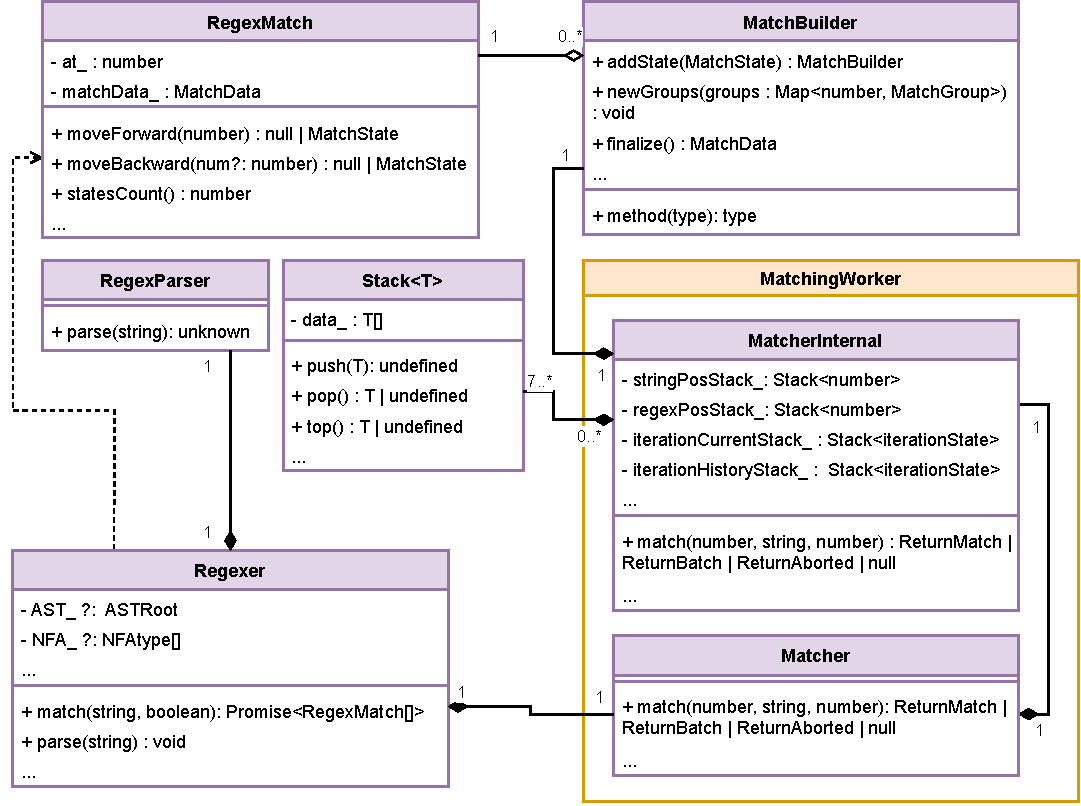
\includegraphics[width=0.9\textwidth]{Figures/UML_RGXR.pdf}
	\caption{Třídní diagram části knihovny pro práci s regulárními výrazy}
	\label{fig:ARCH_RGXR}
\end{figure} 

\section{Parsování regulárních výrazů}\label{sec:Parse}

\subsection*{Parser}

Jak již bylo zmíněno, pro parsování regulárních výrazu jsem použil bezkontextovou gramatiku \textit{Peggy}.
Jedná se o pokračování projektu PegJS, ale ten se již dlouho nevyvíjí. 
Jelikož knihovna Peggy je stále aktualizována a má velkou podporu vývojářů, tak jsem zvolil její využití pro tuto práci.

V ukázce~\ref{code:grammar1} se nachází vstupní neterminál bezkontextové gramatiky \textit{start}. 
Ten obsahuje výběr mezi dvěma začátky \textit{moded\_start} a \textit{general\_start}.
Výběr je pak dostupný pod názvem \textit{type}, podle toho který se zvolí.
Před dokončením pravidla se na jeho konci může nacházet blok "\{\}", který může modifikovat výsledná data.
Modifikace v rámci pravidla pro začátek probíhá zavoláním instance vlastní třídy \textbf{ParserHandler}, která je součástí gramatiky.
Třída má za úkol zpracovávat příchozí data do struktury, která je ukázaná na obrázku~\ref{fig:JSONex}.

\begin{code}[!ht]
	\begin{minted}{peg}
start 
	= 
	type:(moded_start / general_start)
	{
		const data = { modifiers: type?.modifiers };
		return handler.handle(data, type?.elements, States.ROOT);
	}
	\end{minted}
	\caption{Jednoduché pravidlo gramatiky}
	\label{code:grammar1}
\end{code}

Existuje několik různých vzorů regulárních výrazů.
Každý ze vzorů má pravidla pro možné kombinování s ostatními vzory.
Ukázka kódu~\ref{code:grammar2} obsahuje příklad možných výběrů pravidel, které lze společně kombinovat.
Například možnosti pro iteraci, ve zmíněném kódu \textit{to\_iterate}, obsahují pouze následující vzory, které mohou být opakovány.

\begin{itemize}
	\item Speciální znaky (\textit{escaped\_special}) --- "$\textbackslash s$", "$\textbackslash d$"
	\item Základní znaky (\textit{primitive}) --- "$a$", "$b$", "$0$"
	\item Výběr jakéhokoliv znaku (\textit{any\_character}) -- "$.$"
	\item Skupina (\textit{group}) --- "$()$"
	\item List znaků (\textit{list}) --- "$[a-z]$"
\end{itemize}

V mnoha případech záleží na pořadí výběru z dostupných vzorů, proto je potřeba určit, které možnosti upřednostnit.
Abych vysvětlil, proč je pořadí důležité, vybral jsem si jako příklad \textbf{iteraci} (iteration) a \textbf{výběr} (option).
Zjednodušeně výběr má vyšší přednost, jelikož může mít za potomka iteraci.
Kdyby se neterminál iterace nacházel před neterminálem výběru, tak by došlo k tomu, že by iterace nebyla součástí výběru, v případě, že by se nacházela na pozici první možnosti výběru. 
Neboli byla by dříve zpracována, nežli samotný výběr.
Jako příklad může sloužit výraz $a*|b*$, při kterém by se první zpracovala iterace $a*$.
Výsledkem výběru by byly dvě možnosti $\epsilon$ nebo $b*$, což je sice sám o sobě správný tvar výběru, ale ve zvoleném výrazu \textbf{musí} být výsledný výběr $a*$ nebo $b*$.

\begin{code}[!ht]
	\begin{minted}{peg}
any_element 
	= option / iteration / optional / general

to_iterate
	= escaped_special / primitive / any_character / group / list
	\end{minted}
	\caption{Výběry neterminálů pro některé vzory regulárních výrazů}
	\label{code:grammar2}
\end{code}

\subsection*{Struktura zpracovaného regulárního výrazu}

Pro zpracovaný regulární výraz jsem zvolil strukturu, která obsahuje \textbf{nedeterministický konečný automat} (NKA), zároveň s \textbf{abstraktním syntaktickým stromem} (AST).
AST pak slouží k dohledání informací o původním regulárním výrazu. 
Výsledná struktura je objektem, který obsahuje pouze data a má výchozí prototype\footnote{https://developer.mozilla.org/en-US/docs/Learn/JavaScript/Objects/Object\_prototypes}.
Tuto strukturu je možné vidět na obrázku~\ref{fig:JSONex}.
NKA je ve formě \textbf{přesunové tabulky (transition table)}. 
Ta má tvar pole, kde každá položka obsahuje informaci o konkrétním stavu a přesunech na další stavy.
Stav je identifikovaný na základě indexu v poli. 
Přesuny jsou pak implementovány tak, že každý stav si uchovává všechny své přesuny, které vedou z daného stavu do stavu jiného.
Každý přesun pak má informaci, o jaký znak přesunu se jedná a na jaký index (stav) v poli odkazuje. 

Na obrázku~\ref{fig:JSONex} lze vidět výslednou strukturu pro výraz $a+$, která obsahuje dva atributy AST a NFA.
Klíč NFA odkazuje na pole stavů přesunové tabulky. 
AST má odkaz na počátek struktury, který signalizuje začátek regulárního výrazu.
Je zde patrné, že každý stav v tabulce přesunů má odkaz na odpovídající prvek v AST. 
AST prvek/vzor drží různé informace, např. pozice v původním řetězci (start a end), 
potomky daného stavu nebo typ vzoru. 
Ne každý stav musí mít potomky, ale například skupina potomky má.
Některé vzory, jako je například iterace, obsahují v AST dodatečné informace, jako je rozsah iterace (range).
Typy stavů jsou číselné hodnoty, a ty které se nacházejí na obrázku jsou zde také popsány.

\begin{figure}[!h]
	\centering
	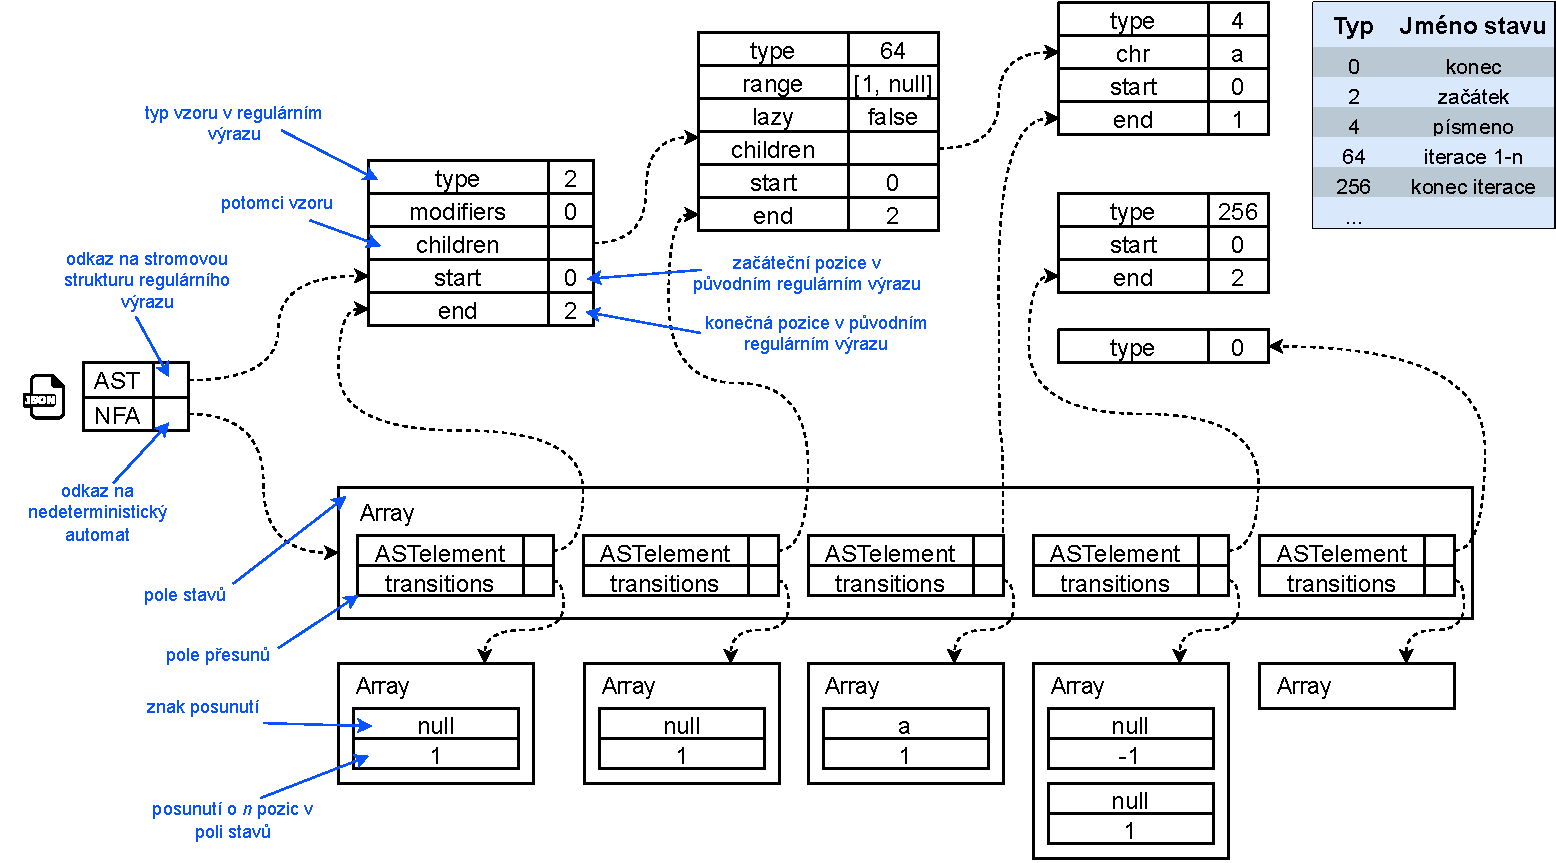
\includegraphics[width=1\textwidth]{Figures/BP-JSON.pdf}
	\caption{Příklad výsledné struktury regulárního výrazu a+}
	\label{fig:JSONex}
\end{figure}

\newpage

\section{Vyhledání pomocí regulárního výrazu}\label{sec:PatternMatching}

Vyhledání je jednou z hlavních částí této knihovny, jedná se o procházení regulárním výrazem a hledaným řetězcem.
Výsledkem je struktura dat, která obsahuje informace o zpracovaném vyhledávání.
V této části textu popisuji, jak jsem naimplementoval vyhledávání, důležité koncepce a výslednou strukturu.

\subsection*{Odstranění rekurze}

Rekurze je sice důležitým aspektem mnoha programů a dokáže usnadnit některé problémy, ale existují situace kdy se vyplatí jí zbavit.
V první řadě, bych rád vysvětlil, proč je rekurzivní řešení vhodné pro vyhodnocování regulárních výrazů.
Jak jsem již zmínil, tak v regulárním výrazu může dojít k backtrackingu.
Nastane ve chvíli, kdy není možné z daného stavu v NKA, přejít na stav jiný.
V tuto chvíli, dojde k vrácení se v NKA do předchozího stavu a k pokračování vyhledávání pomocí další možné cesty.
Nejjednodušší řešení tohoto případu, je použití rekurze.
Pro představu, přechod značí rekurzivní volání funkce a pokud není možné přejít do dalšího stavu, tak se vrací do předchozího volání funkce.

Rekurzi lze odstranit pomocí zásobníků, nebo-li program si uloží, jen potřebné informace.
Ve chvíli kdy dojde k vrácení se (backtrackingu), tak se odstraní vrch zásobníků.
Důležité tedy je správně řídit správu zásobníků, což může být lehce komplikované.

Úryvek zdrojového kódu~\ref{code:matching1}, obsahuje základní vkládání nově navštíveného stavu do zásobníku.
Přesněji se zde ukládá jak stav, tak také index 0 značící počáteční přesun.
Pokud se stav již nachází na vrchu zásobníku, tak je pouze navýšen index přesunu.

% code pushing new state to stack
\begin{code}[!ht]
	\begin{minted}{typescript}
const nfaState = NFA[<number>this.regexPosStack_.top()] as NFAtype;
let topState = this.statesStack_.top();
if(topState?.state !== nfaState)
	this.statesStack_.push({transition: 0, state: nfaState});
else
	topState.transition++;
	\end{minted}
	\caption{Vložení stavu do zásobníku}
	\label{code:matching1}
\end{code}

Příklad kódu~\ref{code:matching2}, souvisí s předchozí ukázkou. 
Jestli nastane situace, kdy neexistuje žádný další přesun z aktuálního stavu, je vyvolán backtracking.
Metoda \textit{handleBacktracking} se stará o správu backtrackingu.
Převážně se jedná o odebírání vrchů zásobníků, jako je již zmíněný zásobník stavů.
Pokud není vrácená hodnota \textbf{null}, znamená to ukončení nebo pozastavení vyhledání.
K neúspěšnému vyhledání a následnému ukončení dojde, pokud je zásobník stavů vyprázdněný a pozice v hledaném řetězci se nachází na jeho konci.

% code poping state from stack
\begin{code}[!ht]
	\begin{minted}{typescript}
const transitions = (nfaState as NFAState).transitions;
if(transitions.length <= <number>this.statesStack_.top()?.transition)
{
	const returned = this.handleBacktracking();
	if(returned !== null) return returned;
	continue;
}
	\end{minted}
	\caption{Vyvolání backtrackingu, pokud neexistují další přechody ze současného stavu}
	\label{code:matching2}
\end{code}

\newpage

\subsection*{Počítání iterací a prevence nekonečných cyklů}

\begin{figure}[!h]
	\centering
	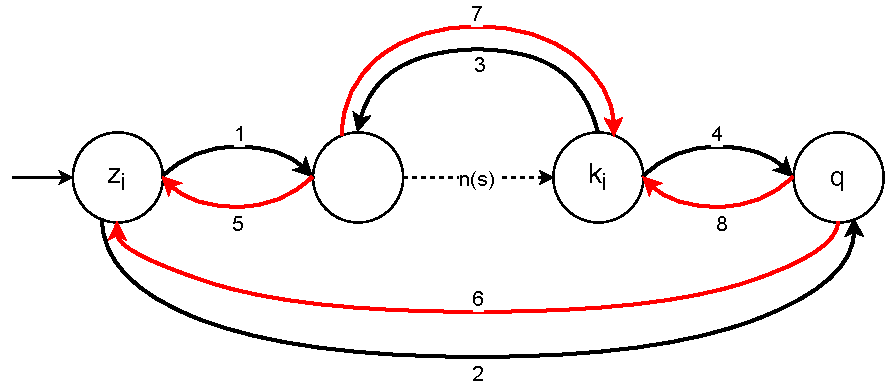
\includegraphics[width=0.65\textwidth]{Figures/IterationCount.pdf}
	\caption{NKA pro popis počítání iterací a prevenci nekonečných cyklů}
	\label{fig:ITERCNT}
\end{figure}

V seznamu pravidel, $I_i$ značí identifikátor iterace, $i$ je počet dokončených opakování iterace a $P_s$ je aktuální pozice v hledaném řetězci.
$I_{arr}$ obsahuje informace v poli o jedné iteraci [$I_i$, $i$, $P_s$].

Algoritmus pracuje se dvěma zásobníky, určenými pro držení informací o iteracích. 
První uchovává aktuálně nedokončené, resp. probíhající iterace. 
Pro popis jej označuji $Z_s$ (zásobník současných iterací).
Druhý značím jako $Z_h$ (zásobník historie), ten slouží pro iterace, které byly již dokončené.
Historie je důležitá pro backtracking.

\begin{enumerate}[label=\arabic* --]
	\item Vlož do $Z_s$ $\longleftarrow$ [$I_i$, 0, $P_s$]
	\item Vlož do $Z_h$ $\longleftarrow$ [$I_i$, 0, $P_s$]
	\item Vrchol $Z_s$, $I_{arr}$[1] + 1
	\item Vlož do $Z_h$ $\longleftarrow$ Odeber ze $Z_s$, $I_{arr}$[1] + 1
	\item Odeber ze $Z_s$
	\item Odeber ze $Z_h$
	\item Vrchol $Z_s$, $I_{arr}$[1] - 1
	\item Vlož do $Z_s$ $\longleftarrow$ Odeber ze $Z_h$, $I_{arr}$[1] - 1
\end{enumerate}

Na obrázku~\ref{fig:ITERCNT} lze vidět nedeterministický automat. 
Jedná se o obecnou reprezentaci iterace, kde $z_i$ reprezentuje začátek iterace, $k_i$ konec iterace a $q$ značí první stav za iterací.
Mezi $z_i$ a $k_i$ se nachází množina stavů $n(s)$.
Červené šipky signalizují backtracking a černé značí klasický přechod mezi stavy.

Jelikož existují iterace v rozmezí, například od 3 do 6, tak je potřeba znát informaci, v kolikátém opakování se právě konkrétní iterace nachází.
Pro tento problém jsem zvolil 8 pravidel, které popisují řešení osmi různých přesunů mezi stavy.
Tato pravidla jsou rozepsána pod obrázkem~\ref{fig:ITERCNT}, indexy pravidel korespondují s indexy v obrázku.
Rád bych poukázal na to, že při backtrackingu se vždy zásobníky vrací, do původních stavů. 
To znamená, mám-li například stavy $a$ a $b$, tak platí pro přesun $a \rightarrow b$ a pro následující backtracking $b \rightarrow a$, že ve stavu $a$ musí být po dokončení obou přechodů hodnoty zásobníků ve stejném stavu jako na začátku.
Jedno opakování je dokončeno při přechodu 3 nebo 4. 
Zároveň přechod 4 společně s přechodem 2, jsou konečnými přechody pro danou iteraci.

Zásobník současných iterací obsahuje poměrně malé množství informací, jelikož se jedná pouze o probíhající iterace.
Naopak zásobník historie může obsahovat poměrně hodně informací. 
Má-li iterace například 100 dokončených opakování, tak historie bude obsahovat minimálně 100 záznamů.
To se může zdát jako mnoho zbytečných informací, ale nelze předem prakticky vědět jestli dojde k backtrackingu a kde se zastaví.

Další důležitou kontrolou, kterou je nutné splnit, je na konci iterace zkontrolovat zda se nachází v určeném rozmezí.
Jelikož počítám jejich opakování, tak stačí tuto informaci porovnat s náležitými mezemi.

V některých případech by mohlo dojít k nekonečnému cyklu.
Například pro regulární výraz $()+$ by k tomu došlo tak, že by nenastalo k posunu v hledaném řetězci, ale přes to by stále procházela úspěšně dále.
K tomu slouží ukládání poslední pozice v hledaném řetězci, při začátku nové iterace, nebo zopakování.
Jestli má dojít k zopakování, musí proběhnou kontrola, zda-li došlo ke změně pozice v řetězci od posledního zopakování.
V obrázku~\ref{fig:ITERCNT} se jedná o stav $k_i$ a přesun $3$.

\subsection*{Využití vlákna pro vyhledávání}
Nedílnou součástí této knihovny je \textbf{paralelní zpracování} v podobě balíčku threads.js.
Balíček byl již zmíněn v kapitole~\ref{sec:USEDtech}.
Pralelismus dovoluje složité operace přesunout do vedlejšího vlákna, aby hlavní vlákno nebylo zatěžováno.
Vlákna sice umožňují efektivnější zpracování náročných programů, ale také mají svá úskalí.

S volbou vývojového prostředí \textit{VSCode}, byla nutnost splnit podmínky stanovené pro práci s web workery, v souladu s jejich API \cite{Microsoft_2021}. 
Podmínkou totiž je, nutnost mít zdrojový kód workeru přímo vložený ve zdrojovém kódu hlavního vlákna.
To znamená, že worker nesmí být přímo načítaný, z adresáře rozšíření.
Avšak tato nutnost, je komplikovaná a proto následovně vysvětlím, jak jsem tento problém řešil.

Všechny závislosti, které worker má, musí být součástí jednoho výsledného souboru.
To je docíleno tím, že přeložím soubor pomocí \textit{webpack}, který vytvoří jeden výsledný soubor.
Pokud by někdo chtěl využít této knihovny, v rámci prostředí NodeJS nebo Prohlížeče, tak tento překlad probíhá dvakrát pro oba runtime.
Tento soubor může následně být vložen přímo do zdrojového kódu.
Pokud aplikace, která využívá tuto knihovnu má webpack, může využít loaderu, který jsem pro tuto knihovnu napsal. 
Ten dokáže v místě kde je worker volaný, vložit jeho zdrojový kód, v rámci textového řetězce.
Výsledkem je worker, který je vložený jako řetězec, ve zdrojovém kódu hlavního vlákna.

Původně tato knihovna zprostředkovávala, pouze paralelismus pro prostředí \textit{NodeJS}.
Později se ale ukázalo, že tato restrikce je limitující, co se týče využití této knihovny ve vizualizační části aplikace.
Regulární výrazy se totiž zpracovávali, na straně rozšíření, které běží v prostředí \textit{NodeJS}.
Vizualizace byla tedy omezena na komunikaci s prostředím, co se týče práce s regulárními výrazy.
Vývojové prostředí pak sloužilo, jako komunikační uzel mezi vizualizací a touto komponentou.
Také toto zprostředkování, poměrně zpomalovalo výkon aplikace, jelikož se musela data posílat pomocí zpráv mezi dvěma komponentami.
Samotná vizualizace, nemohla existovat jako samostatná webová stránka, jelikož zde existovala přímá závislost na rozšíření.
Změnou této části aplikace, která současně podporuje využití paralelismu, pro jakákoliv prostředí, byly tyto problémy eliminovány.

\subsection*{Výsledek vyhledávání}

Výsledkem vyhledávání je třída, obsahující data s informacemi o procházení.
Jejich tvar se neřídí žádným standardem, nebo-li výsledná struktura je čistě přizpůsobená této práci.
Vlastnosti výsledného objektu obsahují všechny důležité informace.
První hodnotou je, zda-li bylo vyhledání úspěšné, či nikoliv. 
Další jsou skupiny, které drží informace, kde se nachází v regulární výrazu a hledaném řetězci. 
Pokud se jedná o pojmenovanou skupinu, tak se také ukládá její jméno. 
Poslední vlastností, která stojí za zmínku je pole, nebo-li seznam všech po sobě jdoucích stavů.

Ve stavech se nachází údaje, které reprezentují historii průchodu.
Každý stav obsahuje, údaj o pozici v řetězci a ve výrazu. 
Také musí být identifikován, o jaký vzor regulárního výrazu se jedná.
Stav může obsahovat další data, která jsou nepovinná, nebo-li se nenachází ve všech stavech.
Jedná se převážně o typ akce a seznam skupin.
Akce je informace, která upřesňuje typ stavu, jako je například backtracking.
Seznam skupin se může nacházet, také v jednotlivých stavech.
Lze pak pozorovat průběh vývoje skupin, s vývojem stavů.

Výsledné stavy se mohou lišit, jak dle počtu, nebo také podle tvaru. 
Modifikace vznikne na základě předem určených nastavení.
Ta například umožňují zahodit nežádoucí informace, nebo naopak přidat rozšiřující.
Zvolil jsem tuto možnost nastavení, aby knihovna mohla být univerzálnější a flexibilnější.

Data jsou uložená v objektu, který je dále součástí třídy \textbf{RegexMatch}.
Samotná třída poskytuje pouze rozhraní pro procházení stavů, nebo popřípadě pro získání dalších základních informací o vyhledávání.

\endinput

% Seznam literatury
\printbibliography[title={Literatura}, heading=bibintoc]

% Prilohy
% TODO: appendix
\appendix

% Priloha vlozena primo do hlavniho LaTeX souboru. Ne vsechny prilohy je nutne mit ve zvlastnich souborech.
% \chapter{Dlouhý zdrojový kód}

\end{document}
